\begin{figure}[htpb!]
\centering
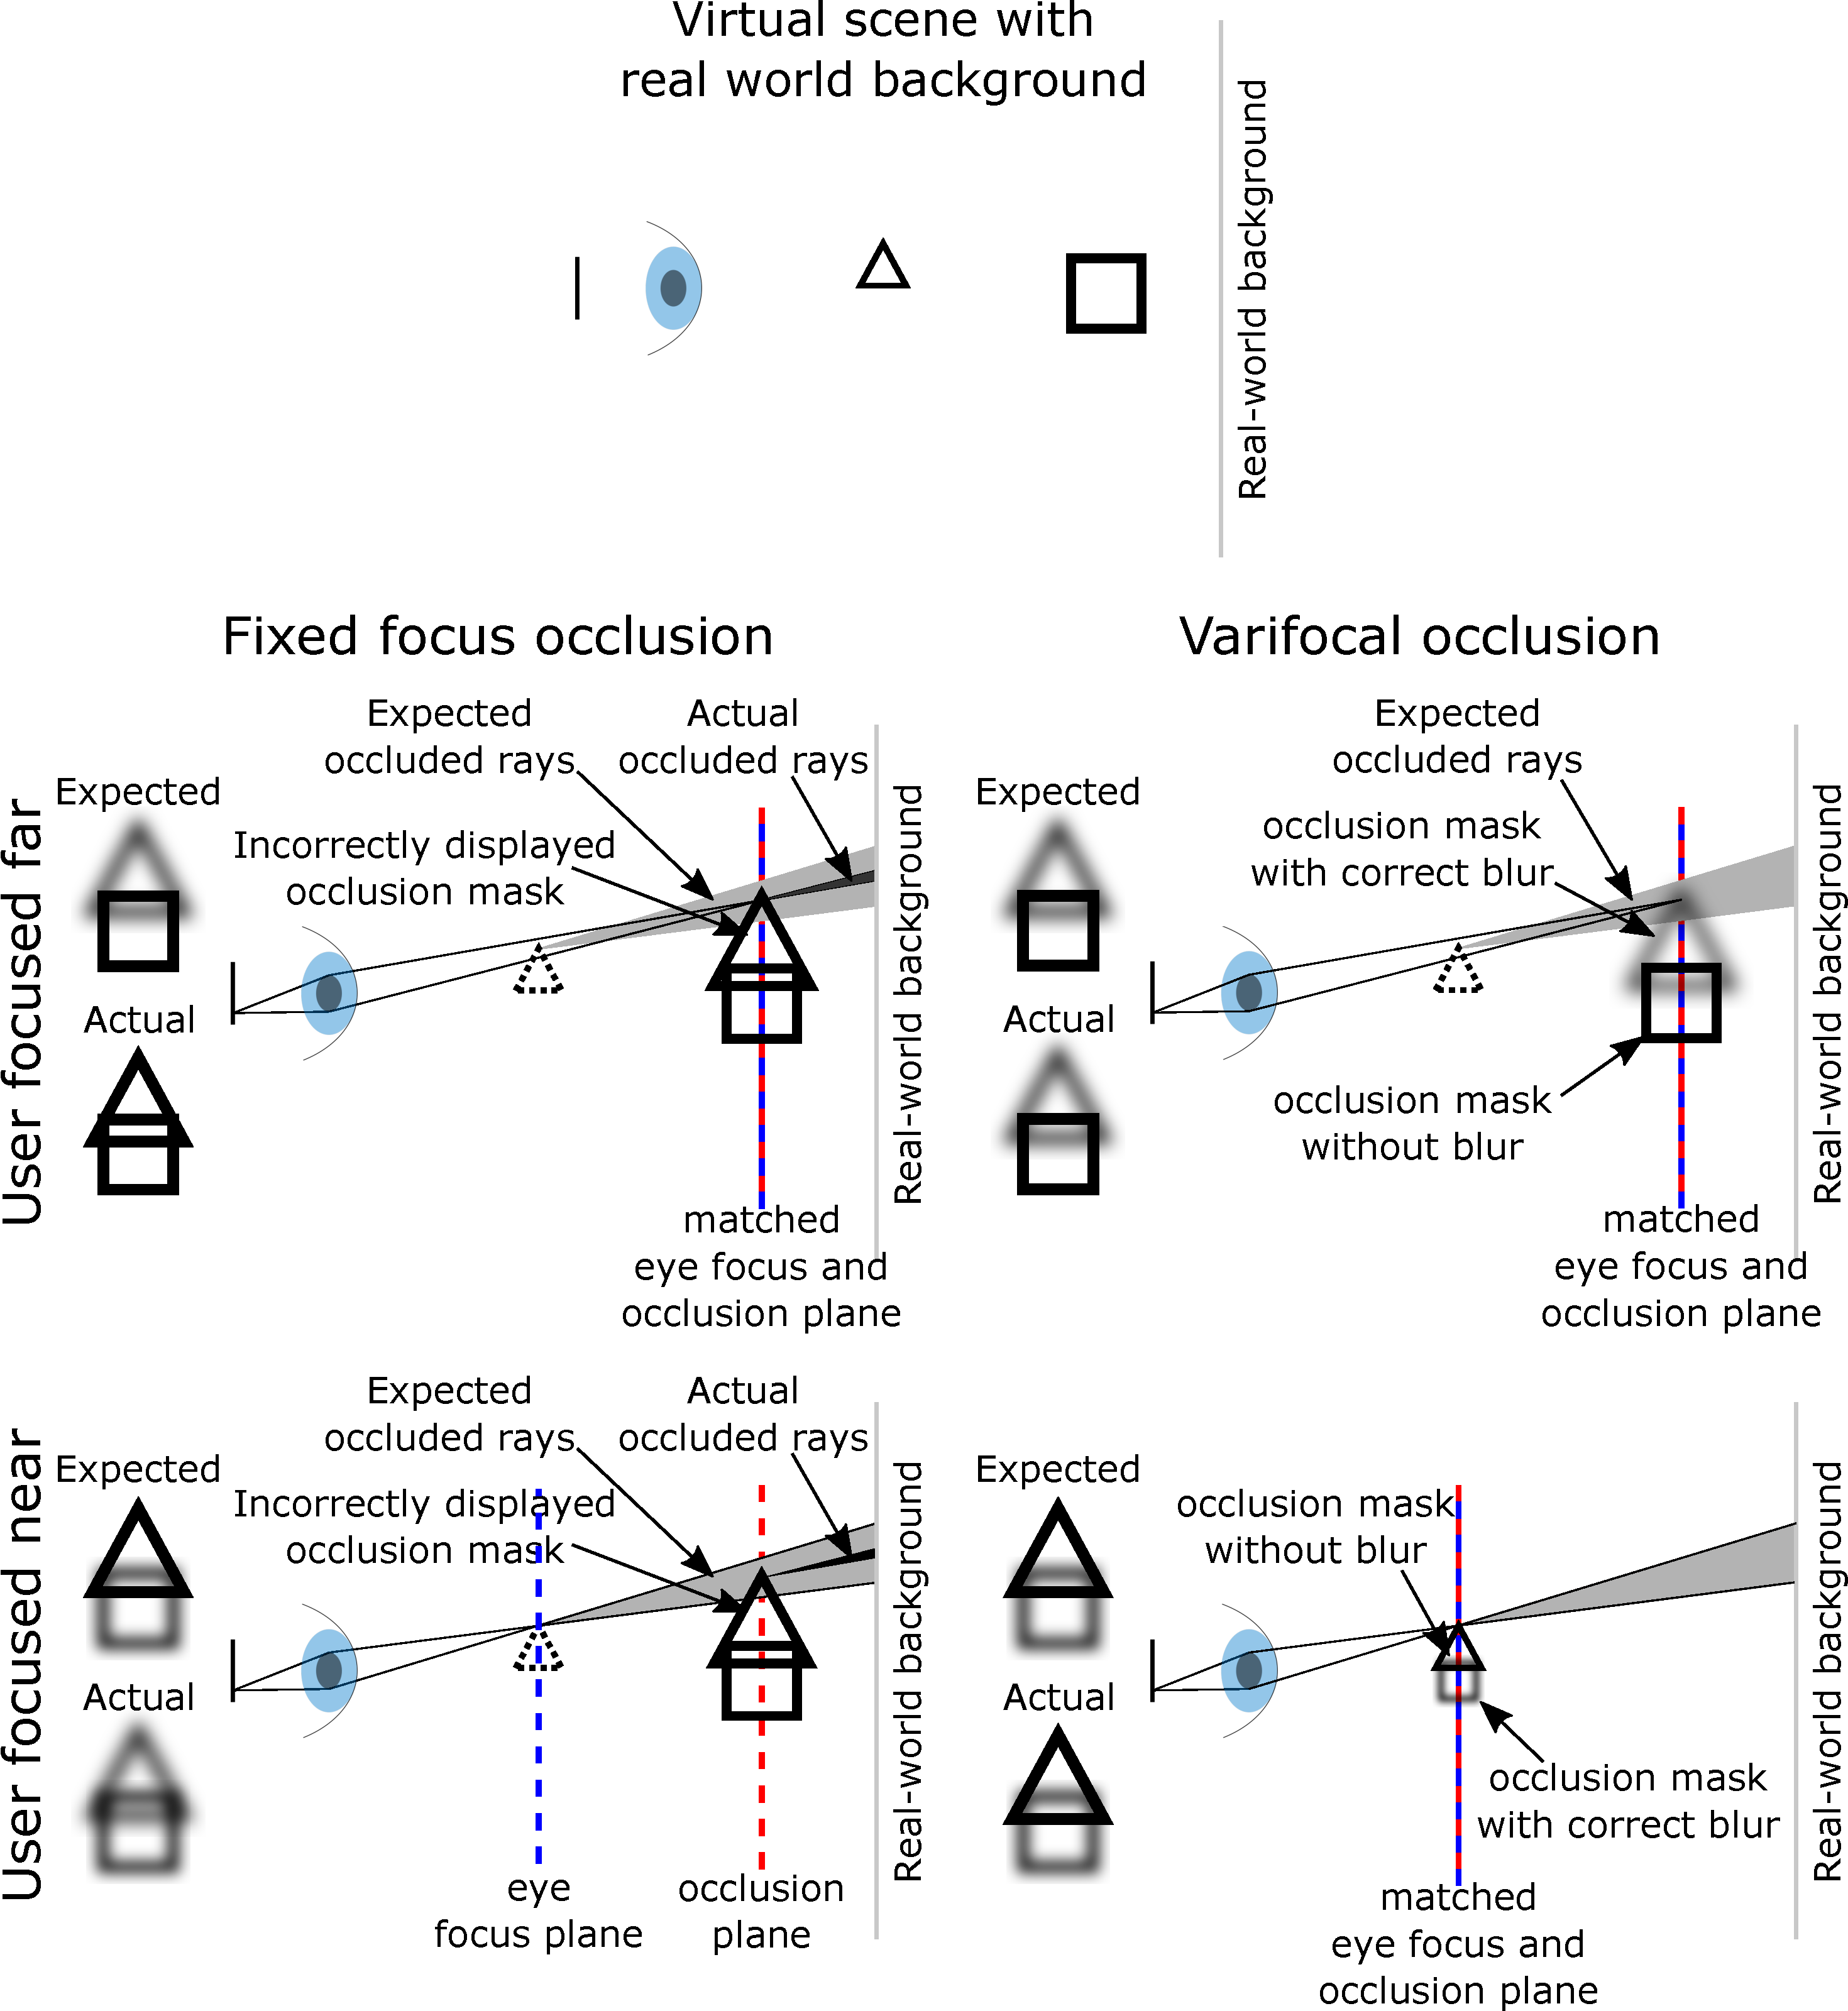
\includegraphics[width=0.9\columnwidth]{images/varifocal_occlusion/depth-dependent-occlusion}
%\fbox{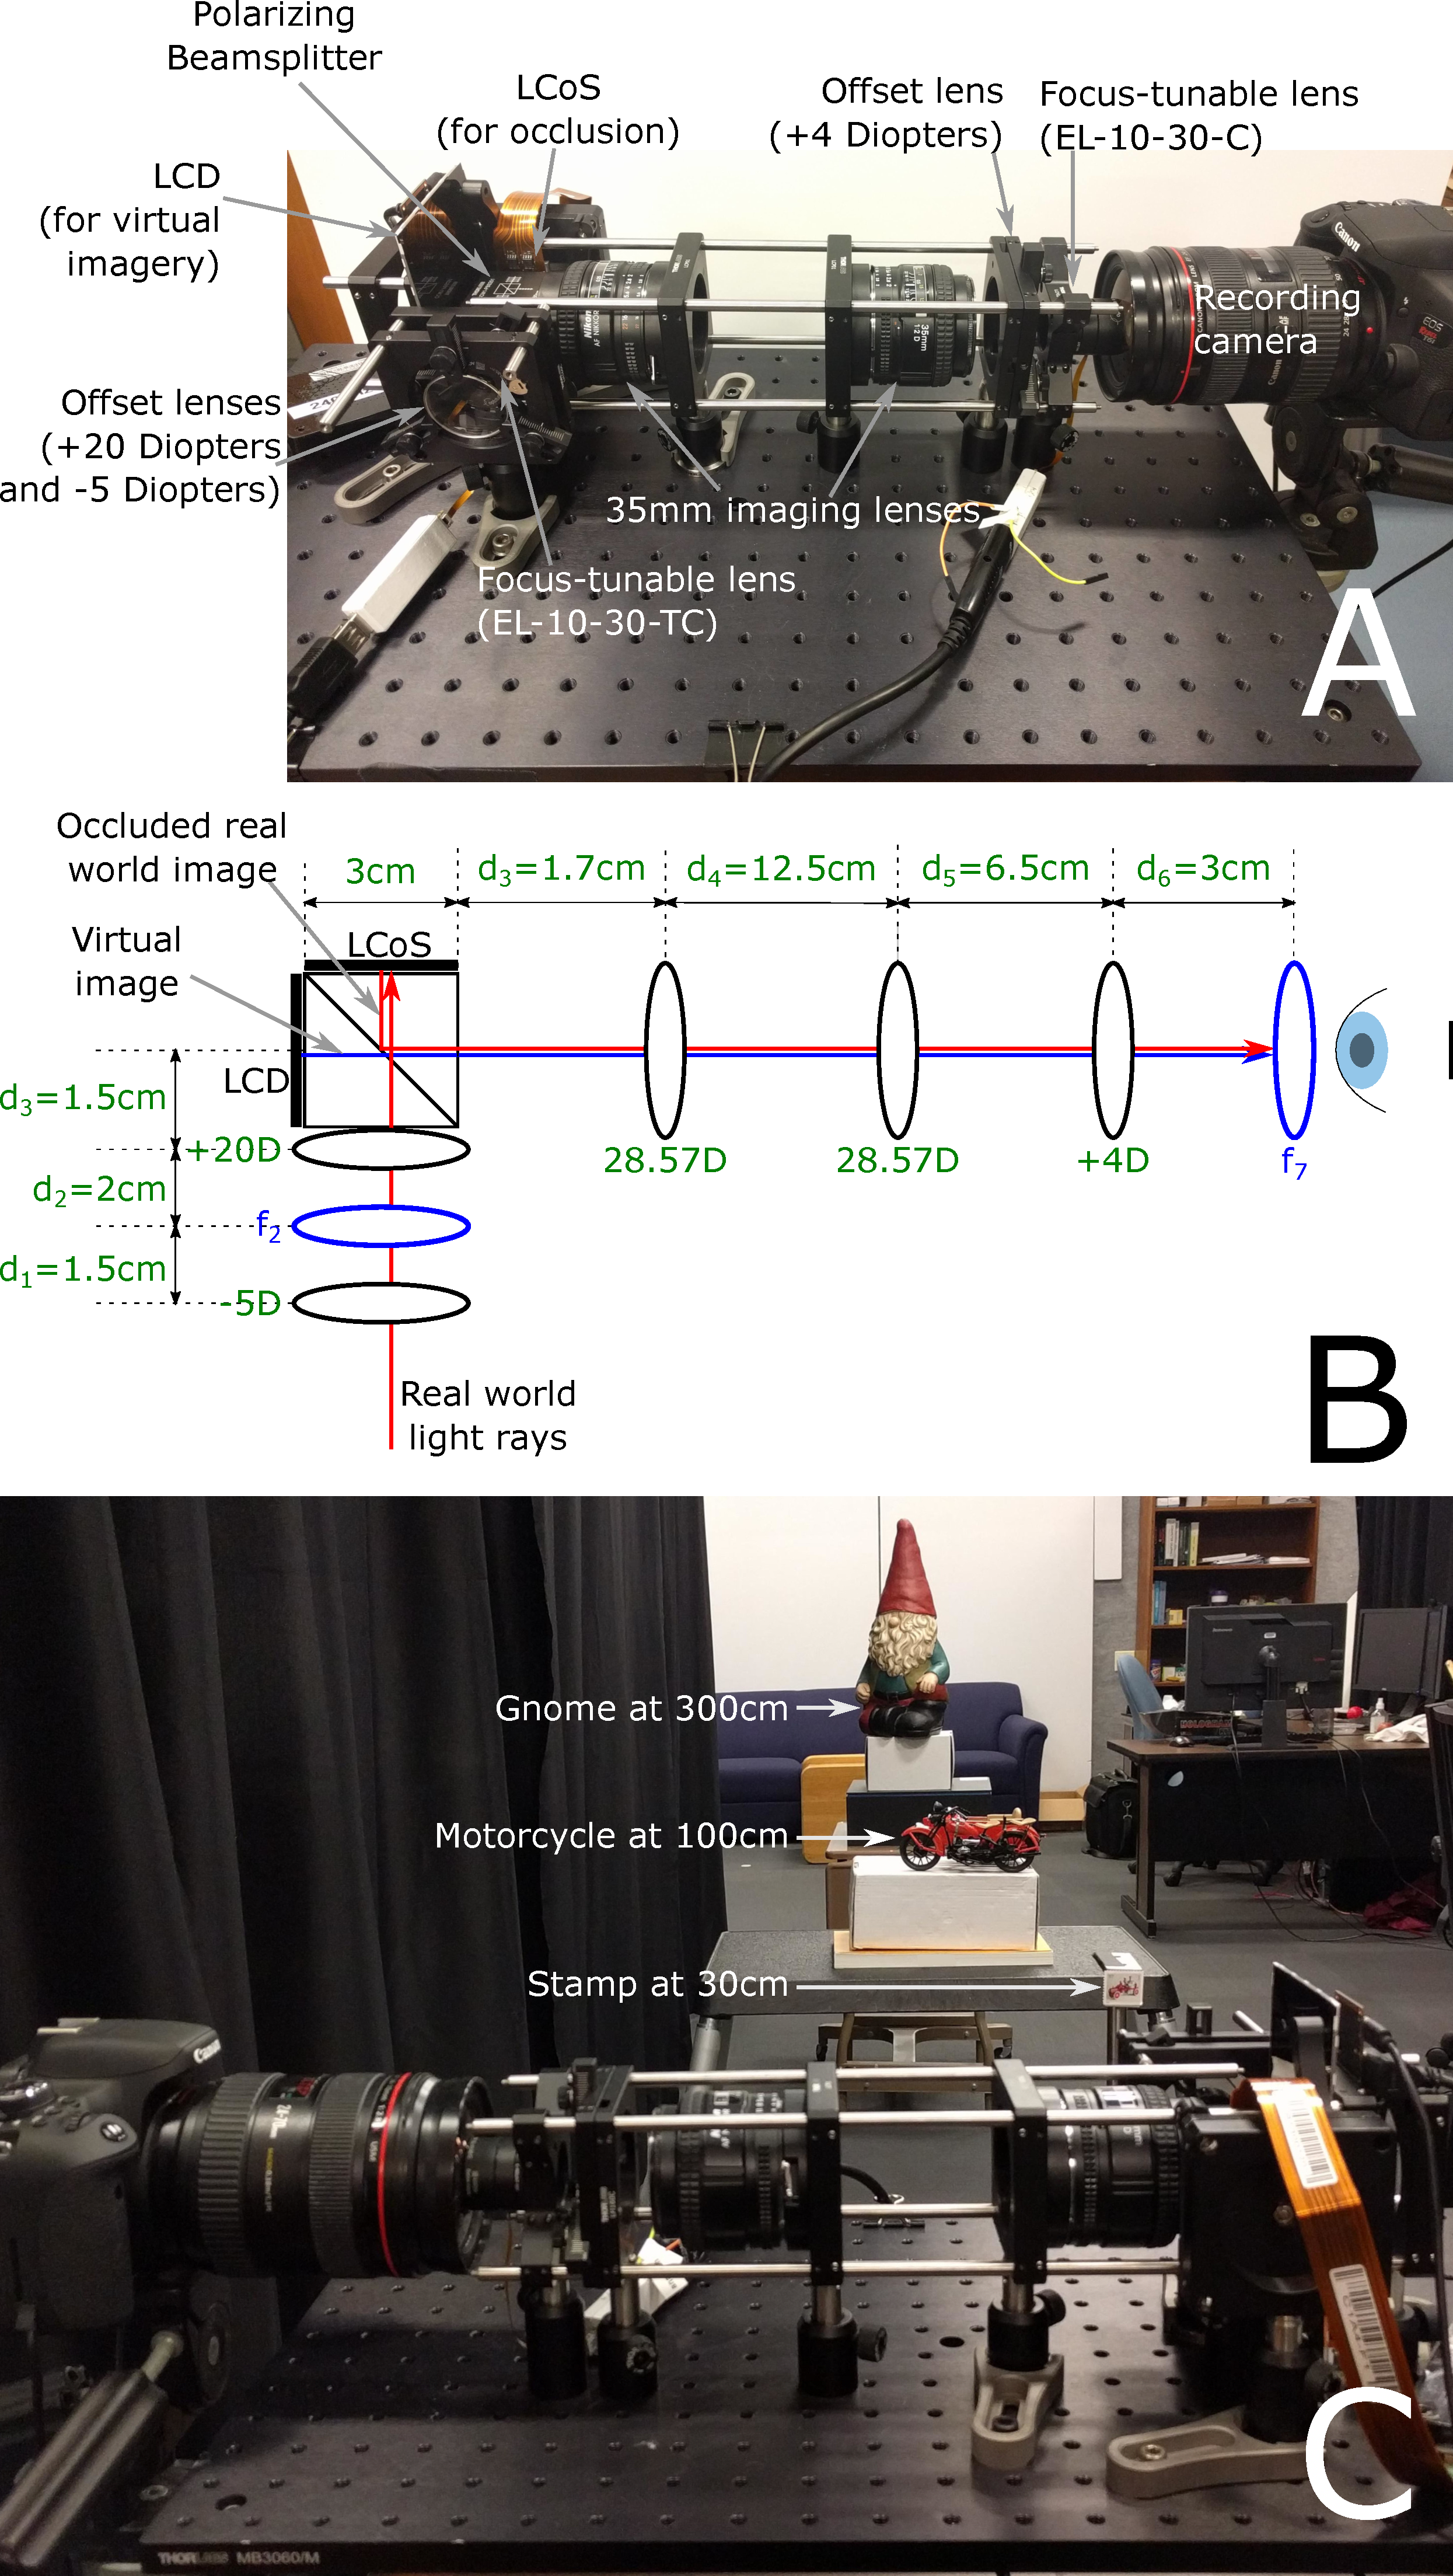
\includegraphics[width=0.46\textwidth]{images/prototype}}
\caption[Varifocal-Occlusion NED: Introducing the concept of depth-dependent occlusion]{\emph{Topmost Row:} A virtual scene composed of one near and one far object placed in front of a real-world background. \emph{Grid of figures:} Comparison of occlusion mechanism only (i.e., ignoring the digital or color image) for fixed-focus and varifocal occlusion displays for the above scene. Dashed blue and red lines indicate the user's focal plane and display's occlusion image plane, respectively. Solid black lines indicate image formation for content placed in the user's focal plane. Images next to the eye show the ``Expected" and ``Actual" images seen by the user. Note that for fixed-focus occlusion, the occlusion plane is always at the far distance which causes the nearby object's occlusion mask to be seen incorrectly always and the far object's occlusion mask to be seen incorrectly when the eye is focused nearby. Varifocal occlusion-capable displays, on the other hand, move the occlusion plane to the user's focal plane and display an occlusion mask for in-focus objects as it is and a perceptually correct occlusion mask for out-of-focus objects by applying a computational blur.}
\label{fig:varifocal_occlusion:depth-dependent-occlusion}
\end{figure}
    
